To make simulated annealing work for switch states
we have to supply the missing functions and values
in \autoref{alg:annealing}.\\
There are many ways to implement the probability function \texttt{p()}. For this work
a probability closely resembling the Boltzmann probability was chosen:

\begin{equation}
    p_c(\Delta E, T) = \begin{cases}
        1 & \text{if} \ \Delta E \leq 1\\
        e^{(-\gamma \Delta E/ T)} & \text{if} \ \Delta E > 1
    \end{cases} 
\end{equation}

where $\gamma$ is a constant that can be tweaked for best optimization performance.
For the energy of the system the scoring function (\autoref{eq:score}) is used:

\begin{equation}
    E = 1 - s
\end{equation}

A new random adjacent switch state is generated with \autoref{alg:ssexp:adjacent}.

\subsection{Annealing results}

\begin{figure}[H]
    \centering
    \begin{tabular}{lrrr}
        \toprule
        & SSS & Best random & Best annealed\\
        \midrule
        Score (x100) & 63.1 & 72.5 & 73.7 \\
        Min. Voltage (V) & 369.5 & 389.5 & 389.5 \\
        Max. cable utilization (\%) & 124.7 & 93.6 & 93.6 \\
        Avg. cable utilization (\%) & 17.0 & 16.6 & 16.2 \\
        Max. transformer utilization (\%) & 66.2 & 62.9 & 54.4 \\
        Avg. transformer utilization (\%) & 35.8 & 33.3 & 33.9 \\
        Toal line losses (kW) & 51.6 & 39.0 & 36.5 \\
        \bottomrule
    \end{tabular}
    \caption{
        Table showing the highest scores obtained through simulated annealing
        and random switch state generation vs. the standard switch sate. Refer
        to \autoref{sec:measures} and to \autoref{sec:score} for an explanation
        of the measures used.
    }
    \label{table:annealing:compare}
\end{figure}

The values for the simulated annealing section where obtained using
the "Suburb 2" area. More information about this grid area can be
found in  \autoref{sec:appendix:suburb2}. A comparison
between the SSS and the optimized switch states
can be found in \autoref{table:annealing:compare}. 

\begin{figure}[H]
    \begin{subfigure}{.5\textwidth}
      \centering
      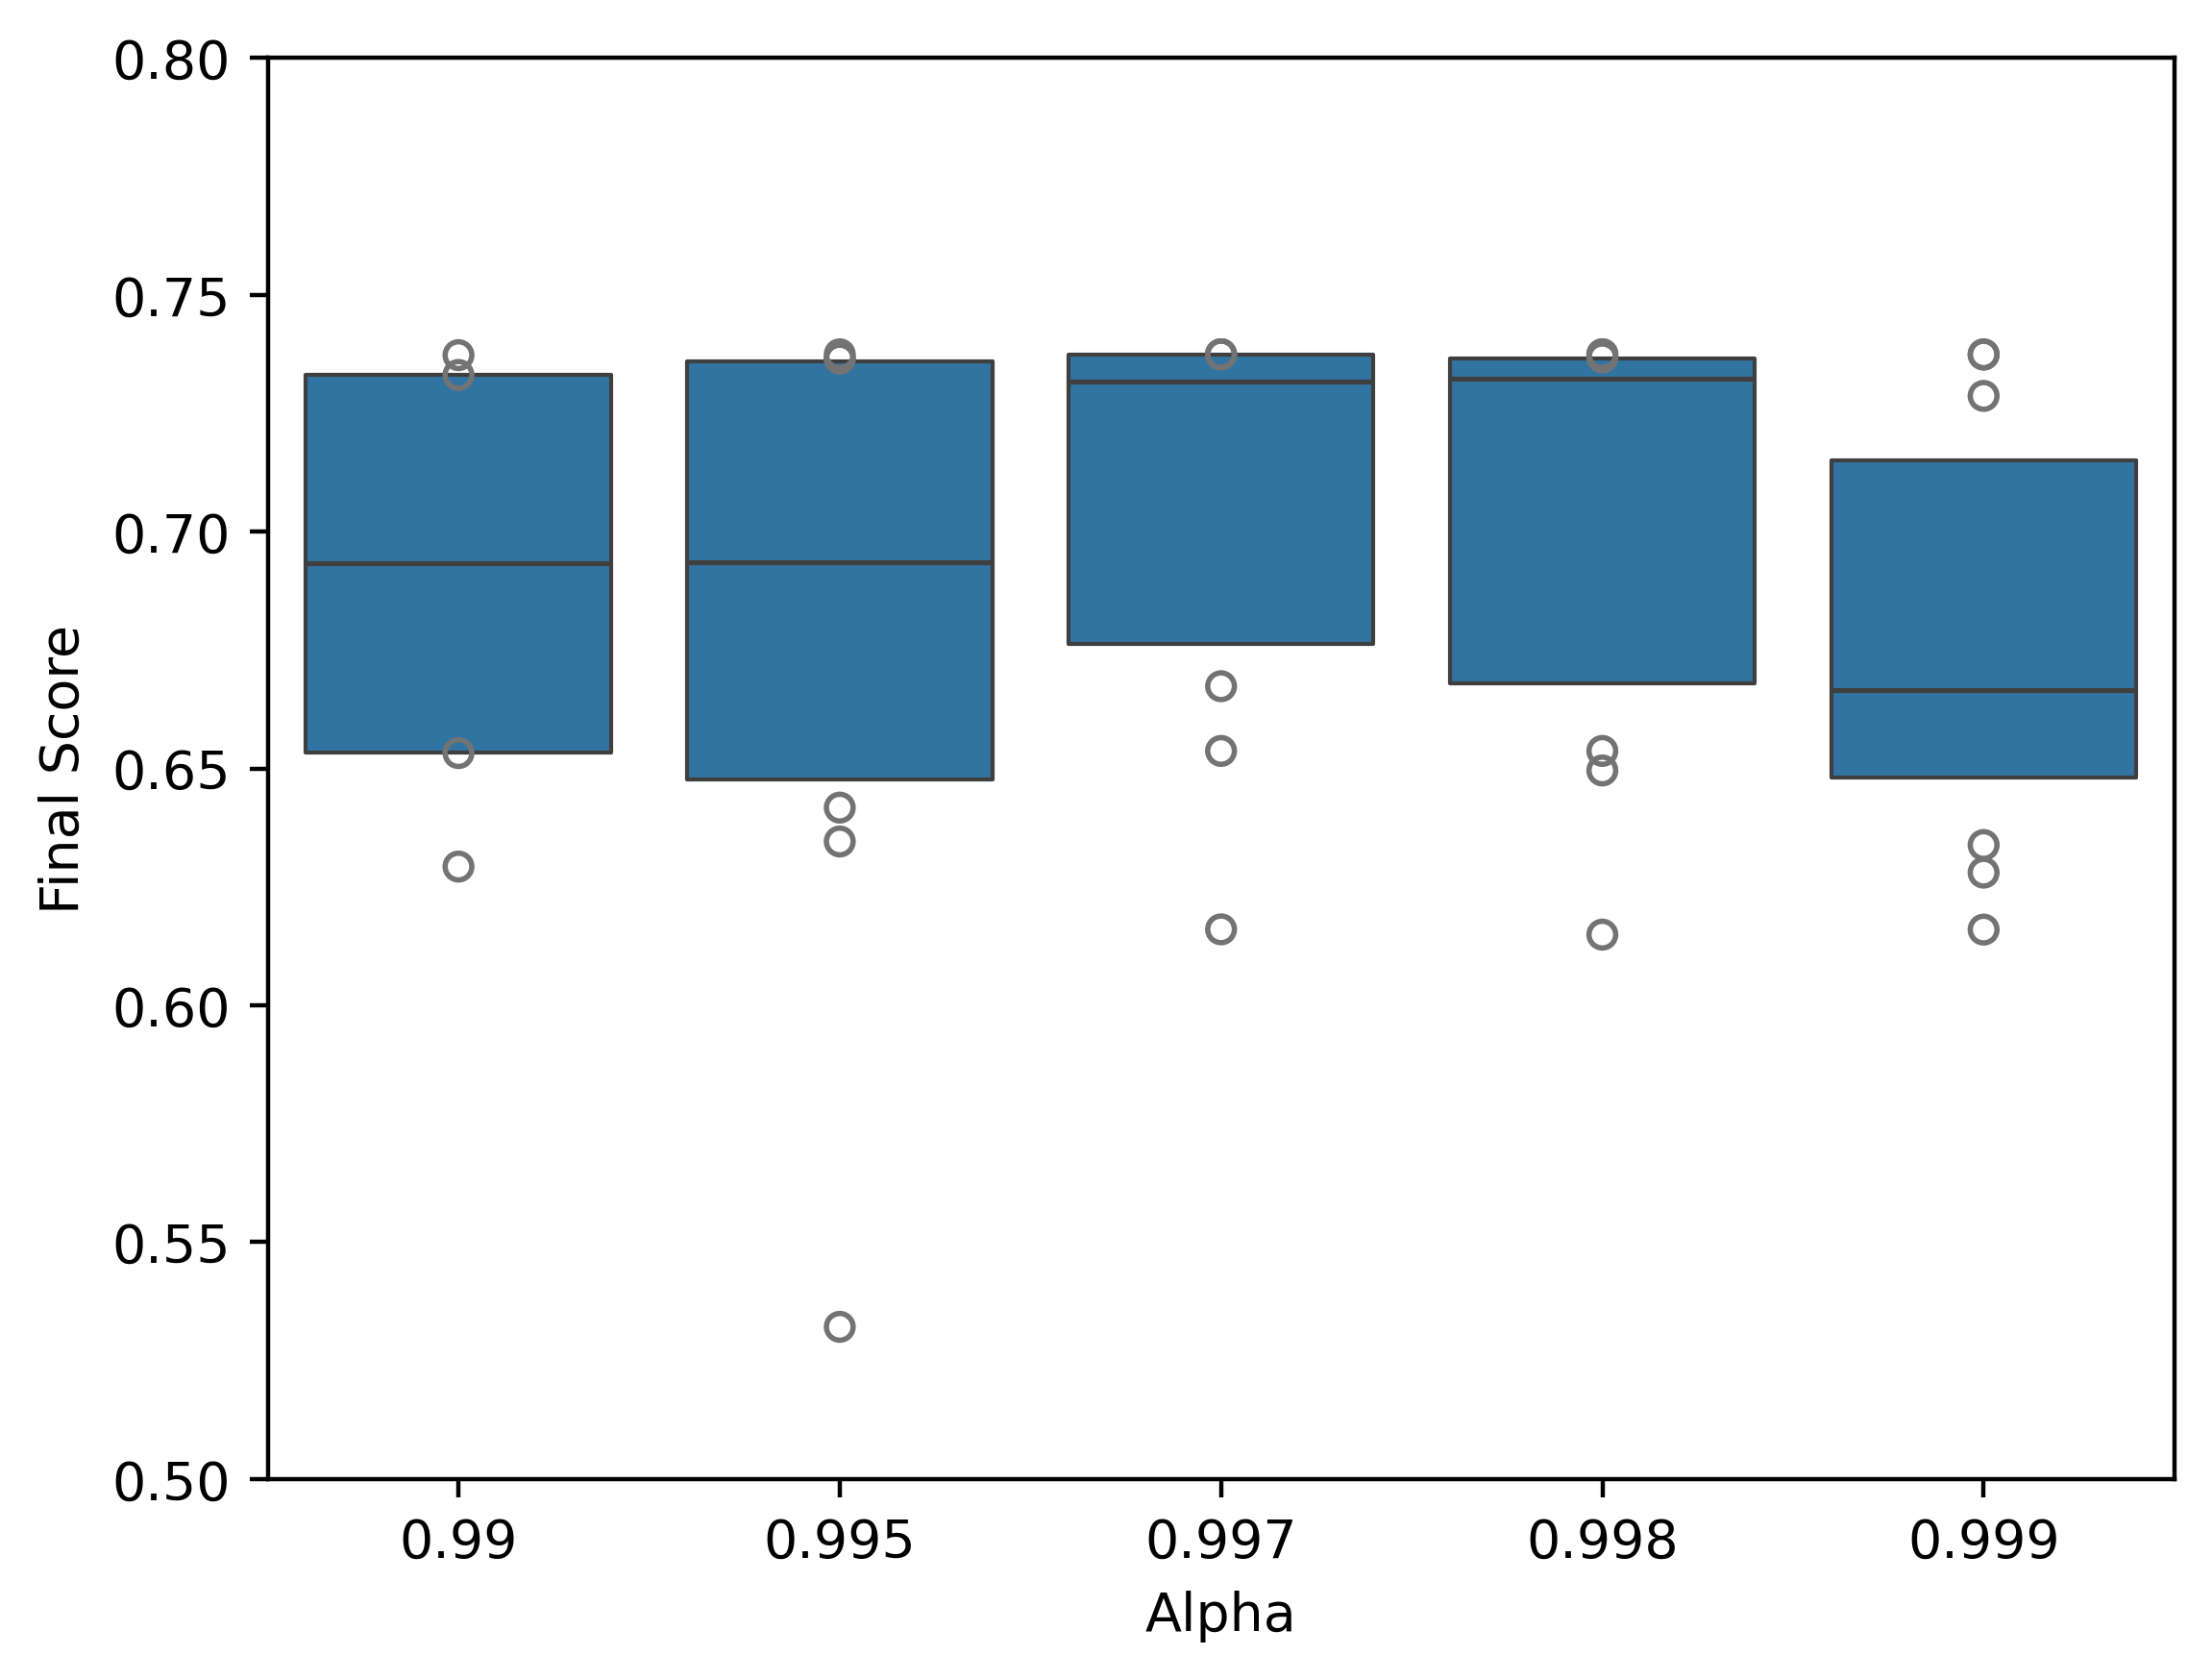
\includegraphics[width=\linewidth]{img/switchstate_exploring/suburb2/annealing_sampling/alhpa.png}
      \caption{}
    \end{subfigure}%
    \begin{subfigure}{.5\textwidth}
      \centering
      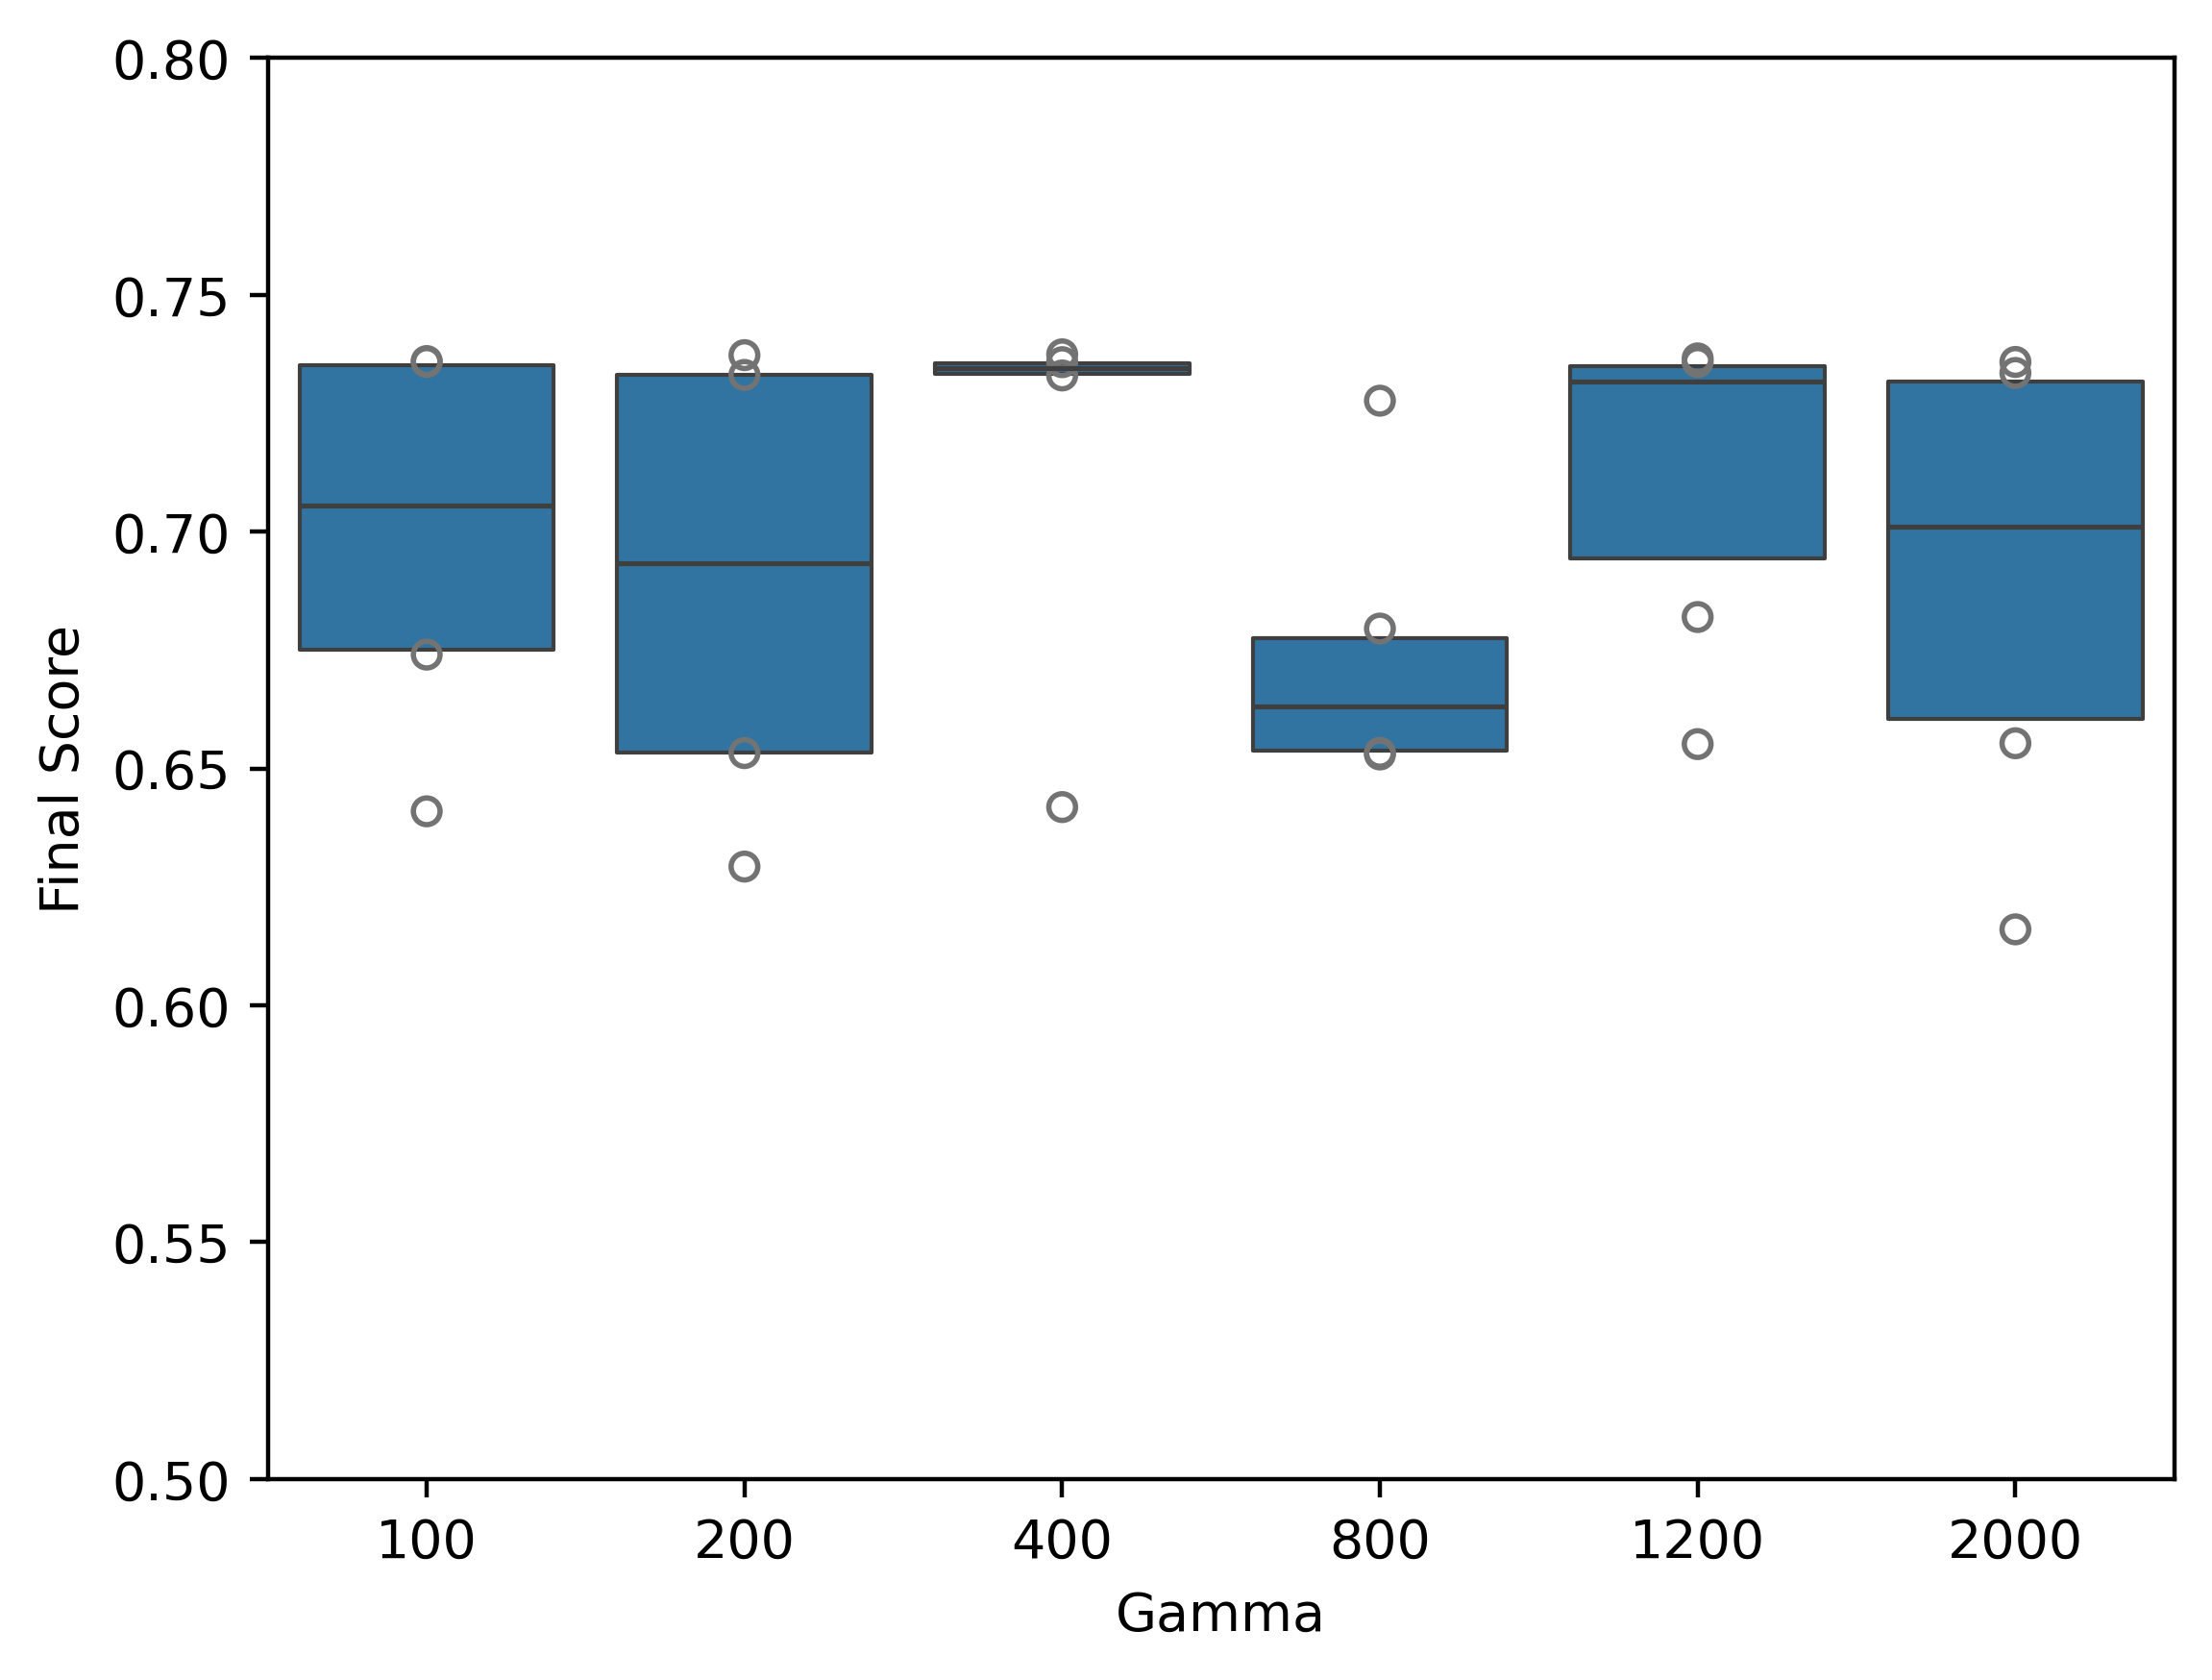
\includegraphics[width=\linewidth]{img/switchstate_exploring/suburb2/annealing_sampling/beta.png}
      \caption{}
    \end{subfigure}\\
    \begin{subfigure}{.5\textwidth}
        \centering
        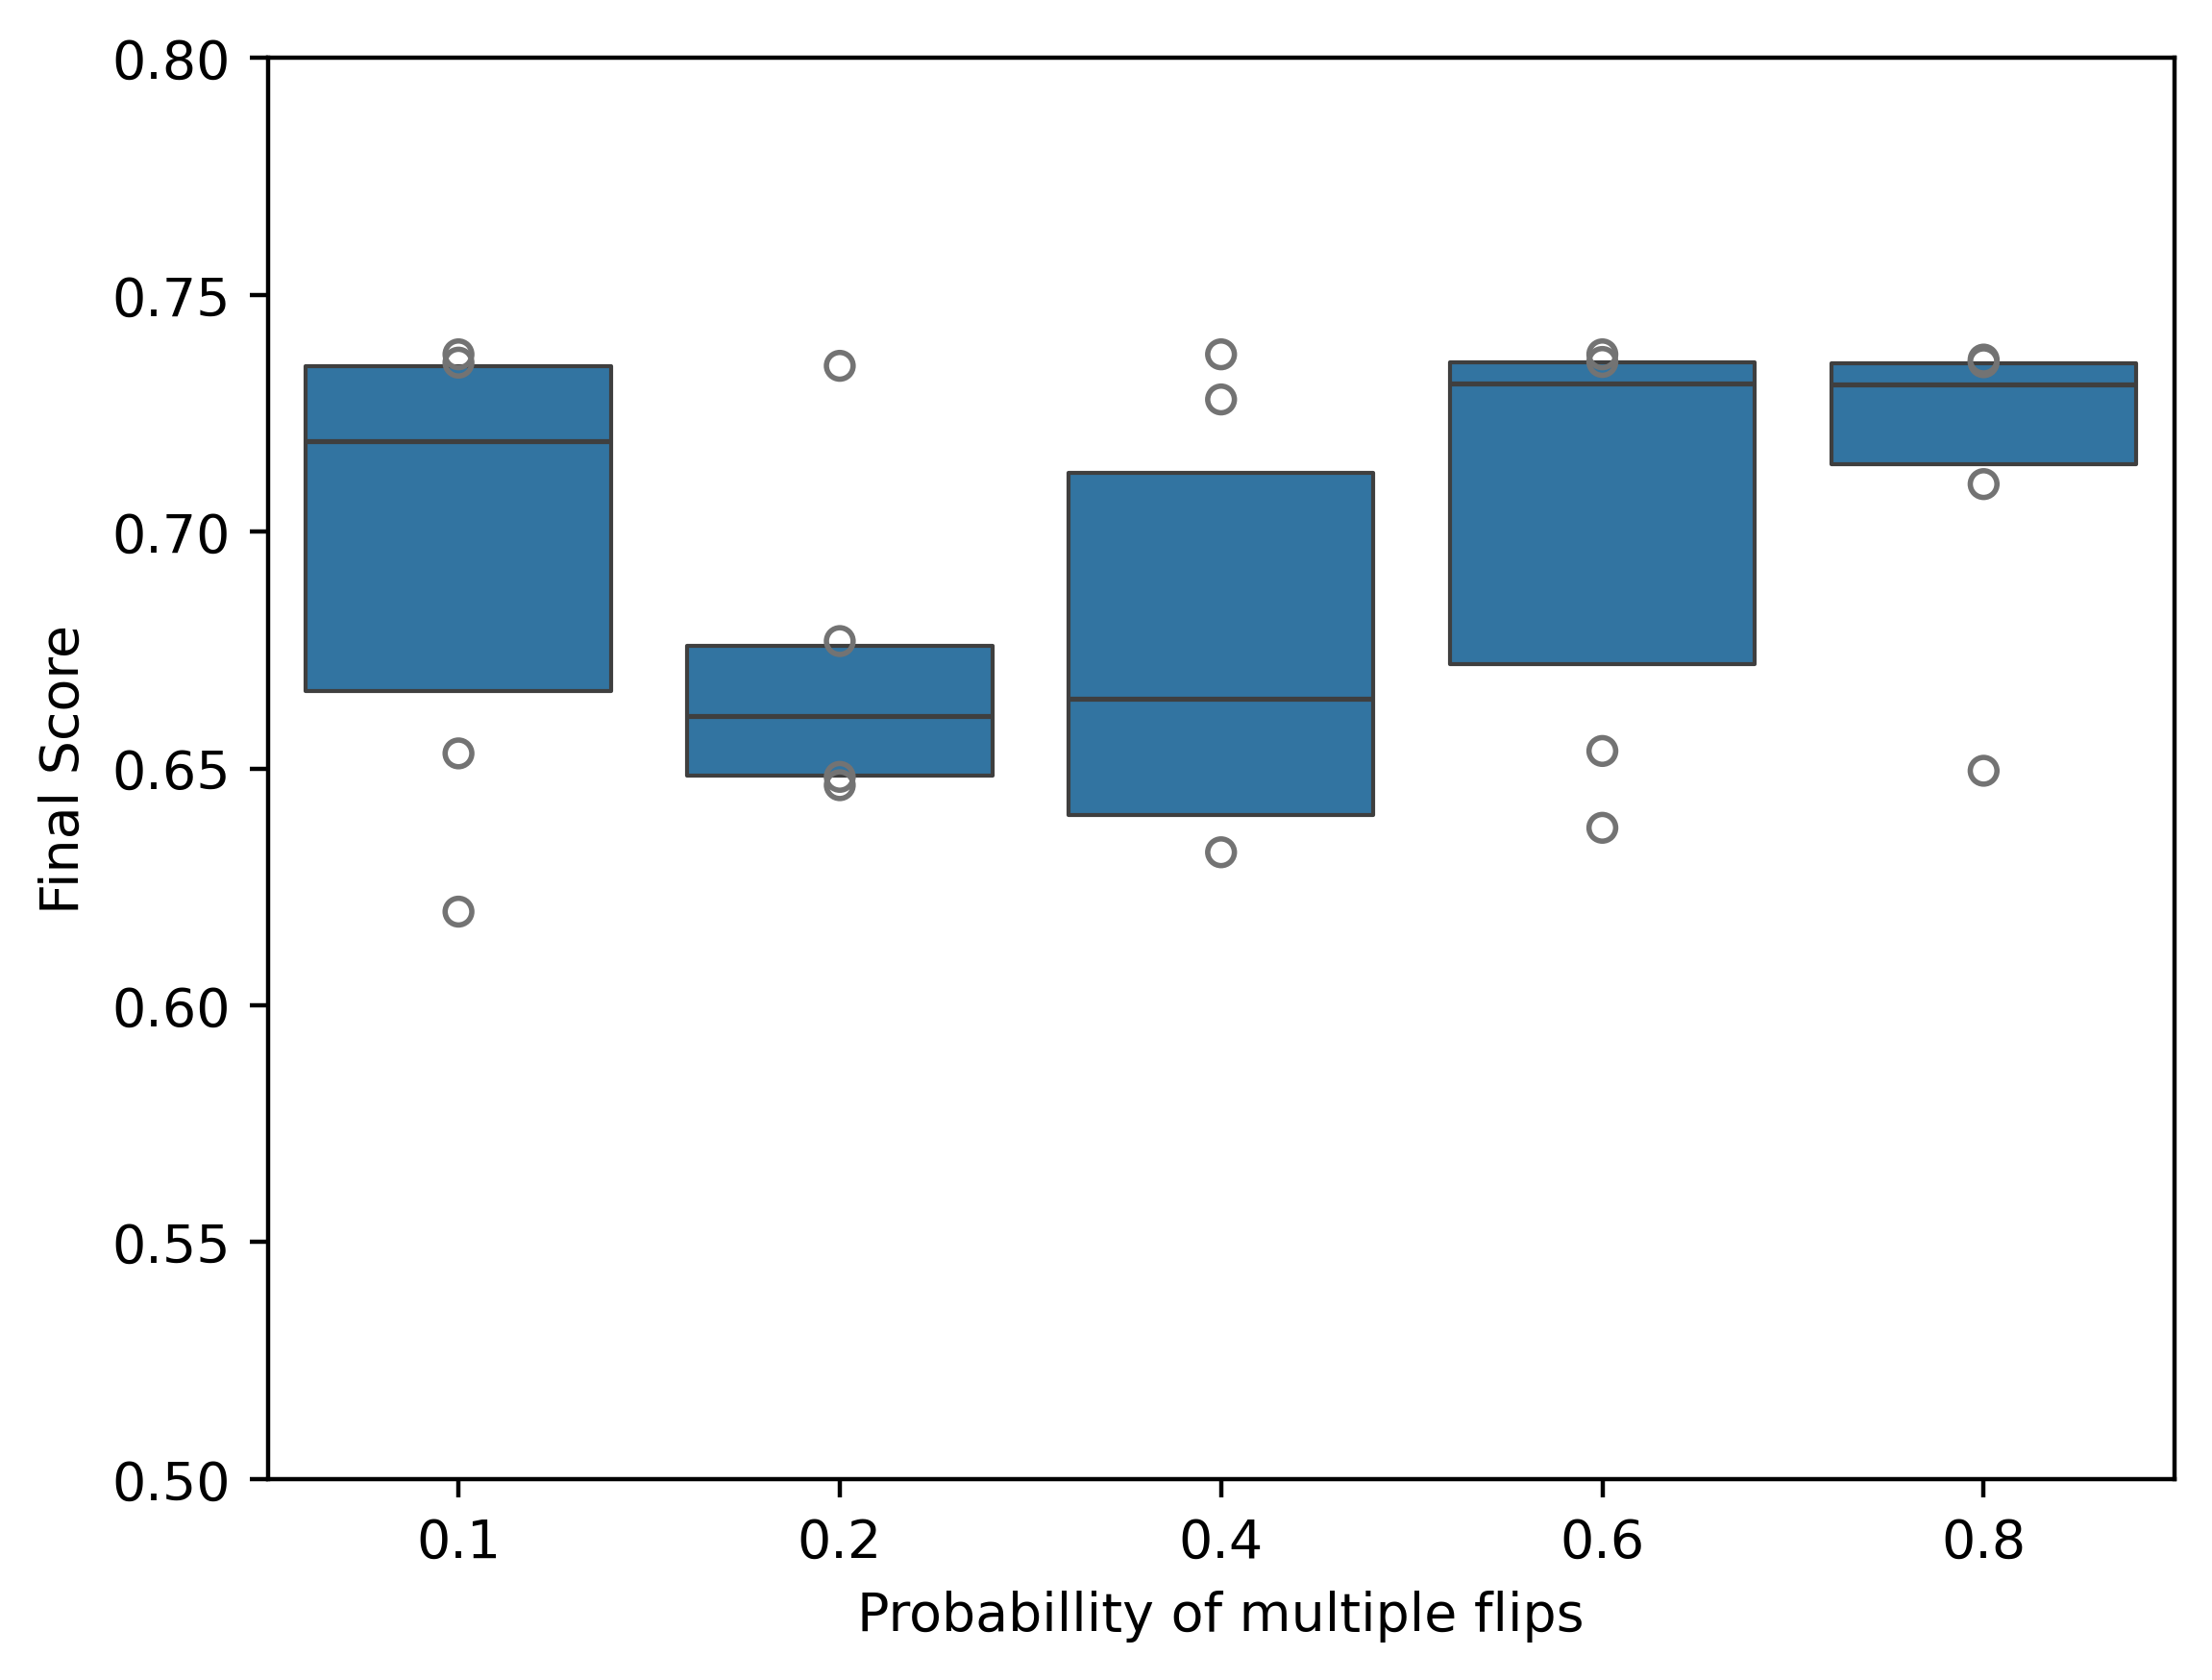
\includegraphics[width=\linewidth]{img/switchstate_exploring/suburb2/annealing_sampling/p_multi.png}
        \caption{}
    \end{subfigure}%
    \begin{subfigure}{.5\textwidth}
        \centering
        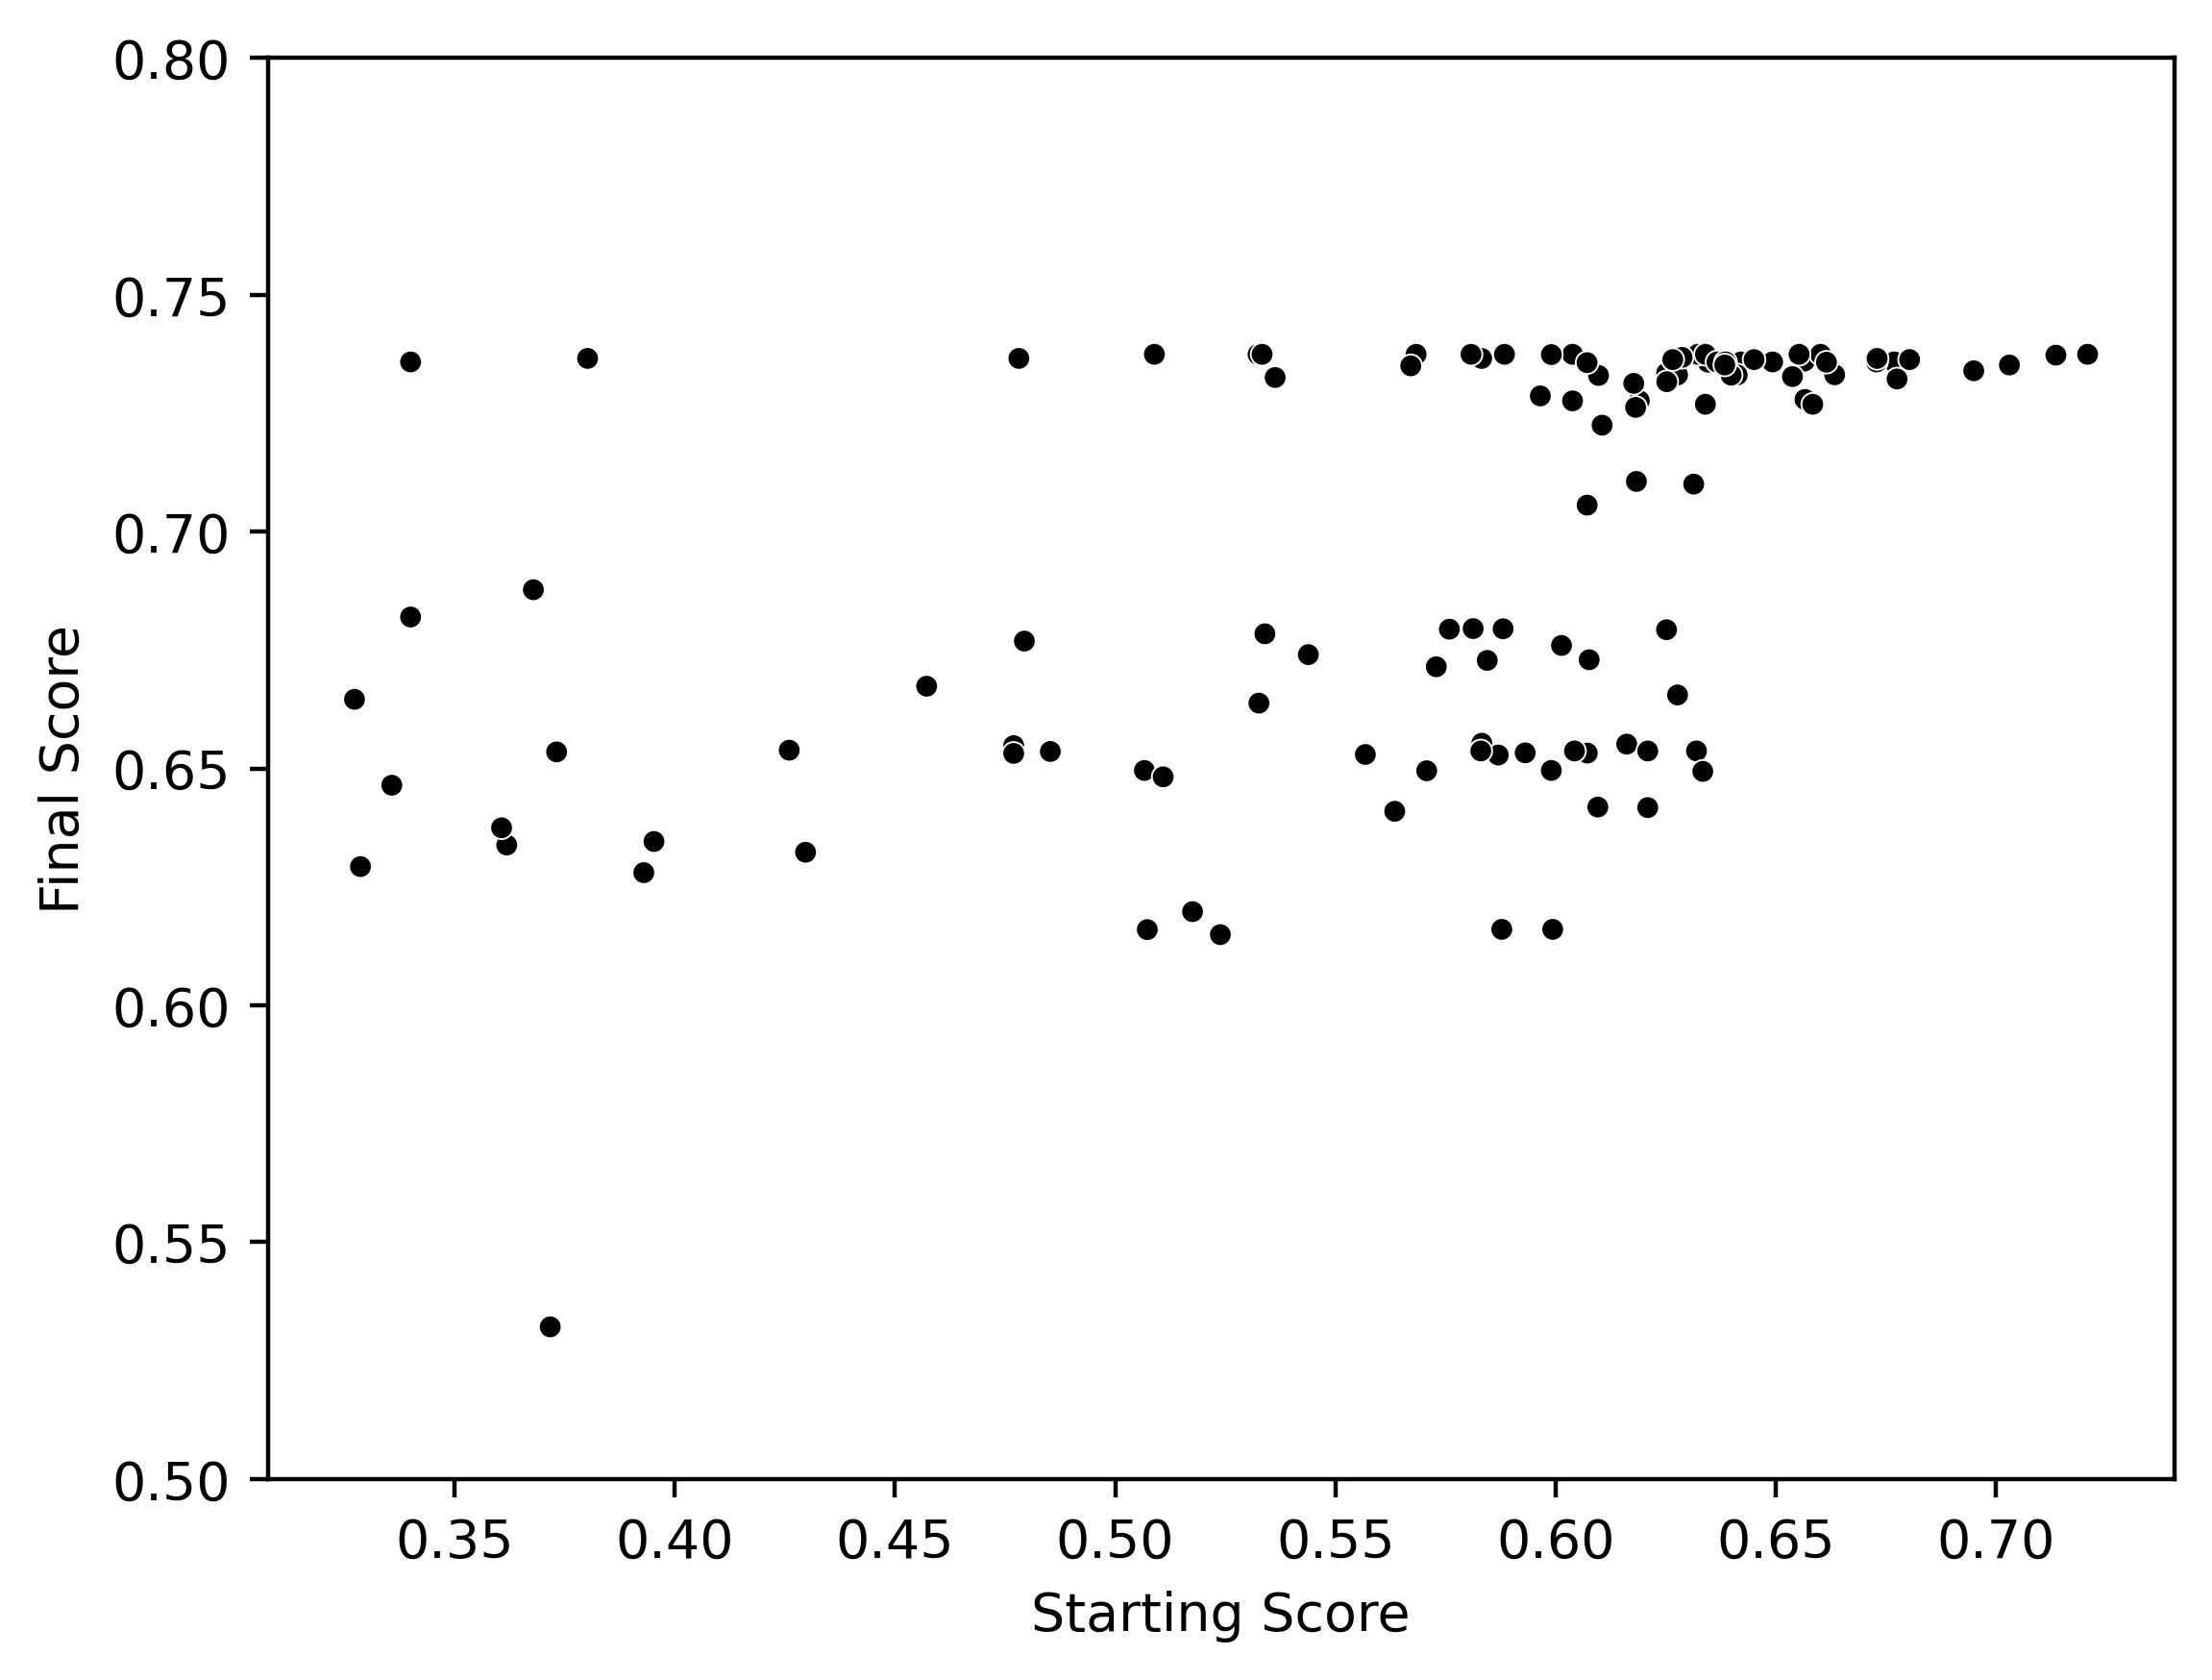
\includegraphics[width=\linewidth]{img/switchstate_exploring/suburb2/annealing_sampling/starting_score.png}
        \caption{}
    \end{subfigure}
    \caption{
        Simulated annealing applied to the "Suburb 2" grid area (\autoref{sec:appendix:suburb2}).
        Plotting score $s$ reached vs. varying values of $\alpha$ (a), $\gamma$ (b), $p_{multi}$ (c) and
        the score of the random switch state configuration that was used as the initial state (d).
        Box plots showing the median, the 25\% quartile, the 75\% quartile and outliers used for (a), (b) and (c).
        6 samples taken for each configuration in (a), (b) and (c). (d) shows all samples of all configurations.
        Initial random switch states where obtained through \autoref{alg:ssexp:random}.
        The standard values where $\alpha = 0.99$, $\beta = 1000$ and $p_{multi} = 0.33$
        when other parameters where examined.
    }
    \label{fig:annealing:parameters}
\end{figure}

\autoref{fig:annealing:parameters} shows the score reached by the annealed grid area
with varying parameterizations and starting switch states. The most surprising result
is that the best score of around $s = 0.75$ can be reached no matter what
the starting switch state is and no matter the parameters chosen. This
seems to suggest that there is an absolute ceiling for the best score that
can be achieved through annealing at that value. This could either be due
to a fundamental limit of the method itself or it could be that this switch
state is actually the optimal switch state and that no better switch state
exists at all. The later conclusion might be supported by the fact that the
four best switch states found are all the same (see \autoref{fig:annealing:topologies})\\
\\
We also cautiously conclude that values of around $\gamma = 400$ and $p_{multi} > 0.8$
make it most probable to reach the maximum score. However, a larger sample size
will be required to determine this. Running the annealing algorithm takes some time
as can be seen in \autoref{fig:annealing:over_time}. Multiple samples have to be taken as
not all trials yield a similar score. 

\begin{figure}[H]
    \begin{subfigure}{.5\textwidth}
      \centering
      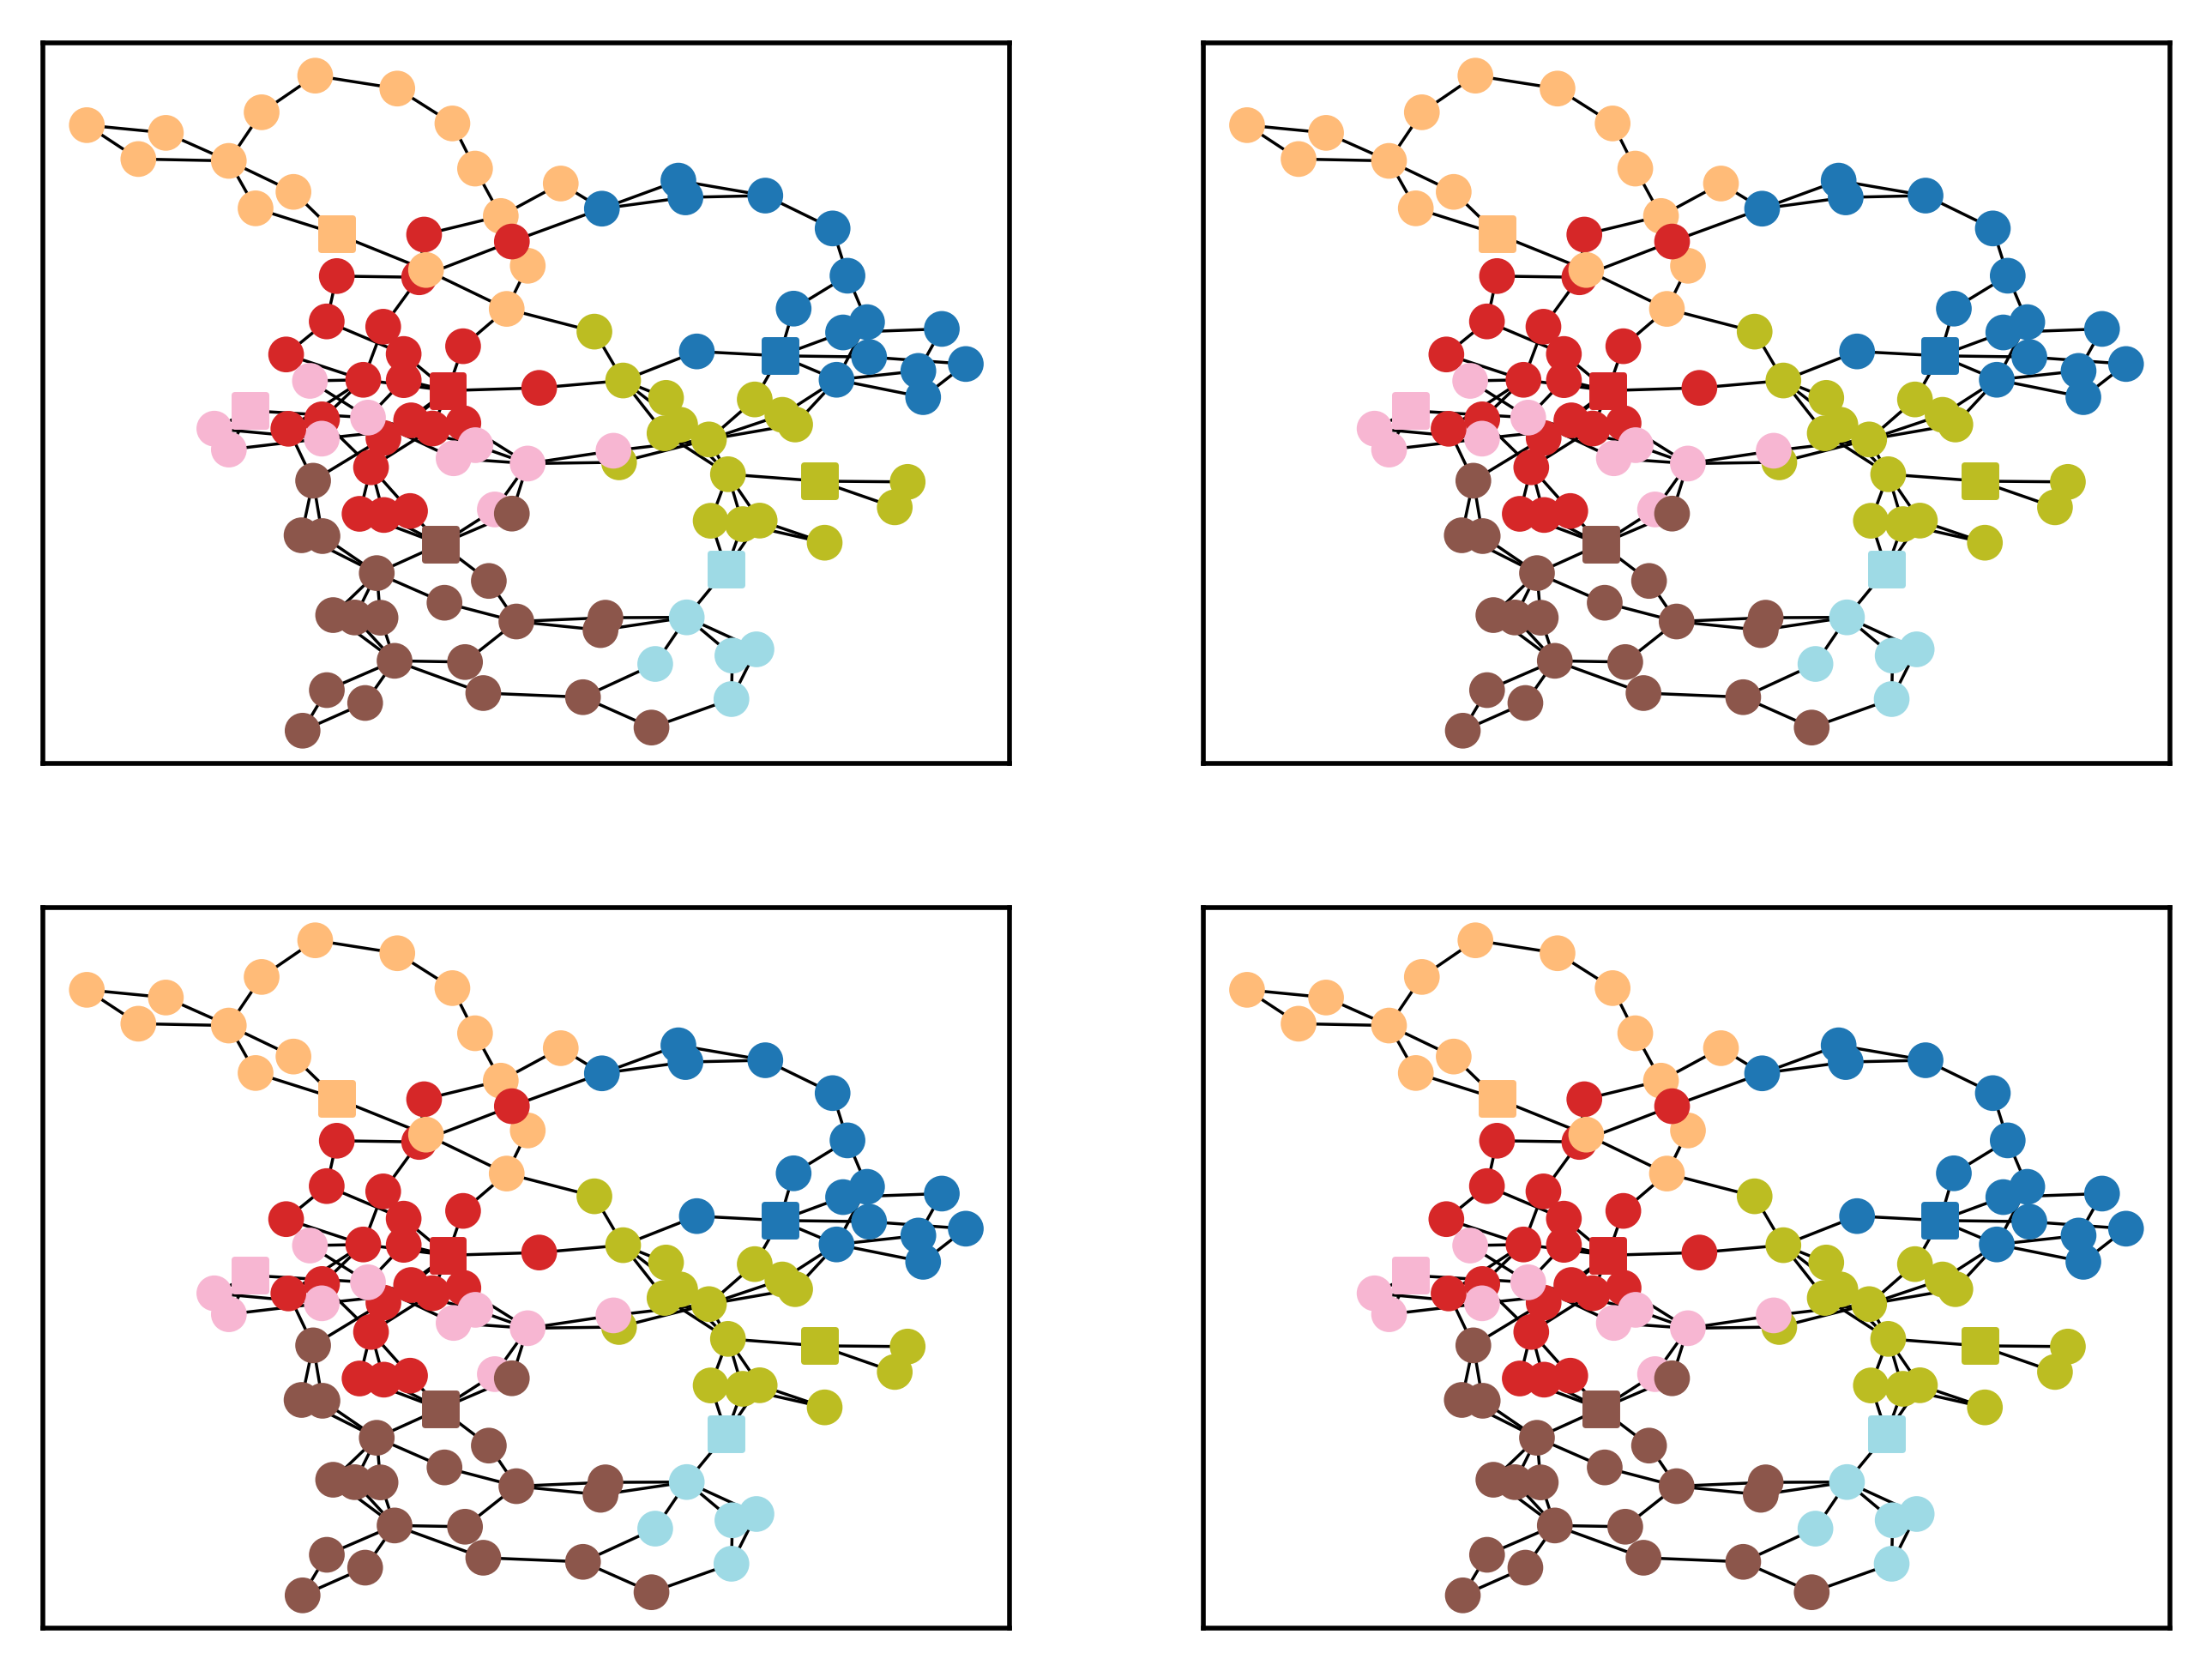
\includegraphics[width=\linewidth]{img/switchstate_exploring/suburb2/annealing_sampling/best_overall.png}
      \caption{
       }
      \label{fig:annealing:topologies}
    \end{subfigure}%
    \begin{subfigure}{.5\textwidth}
      \centering
      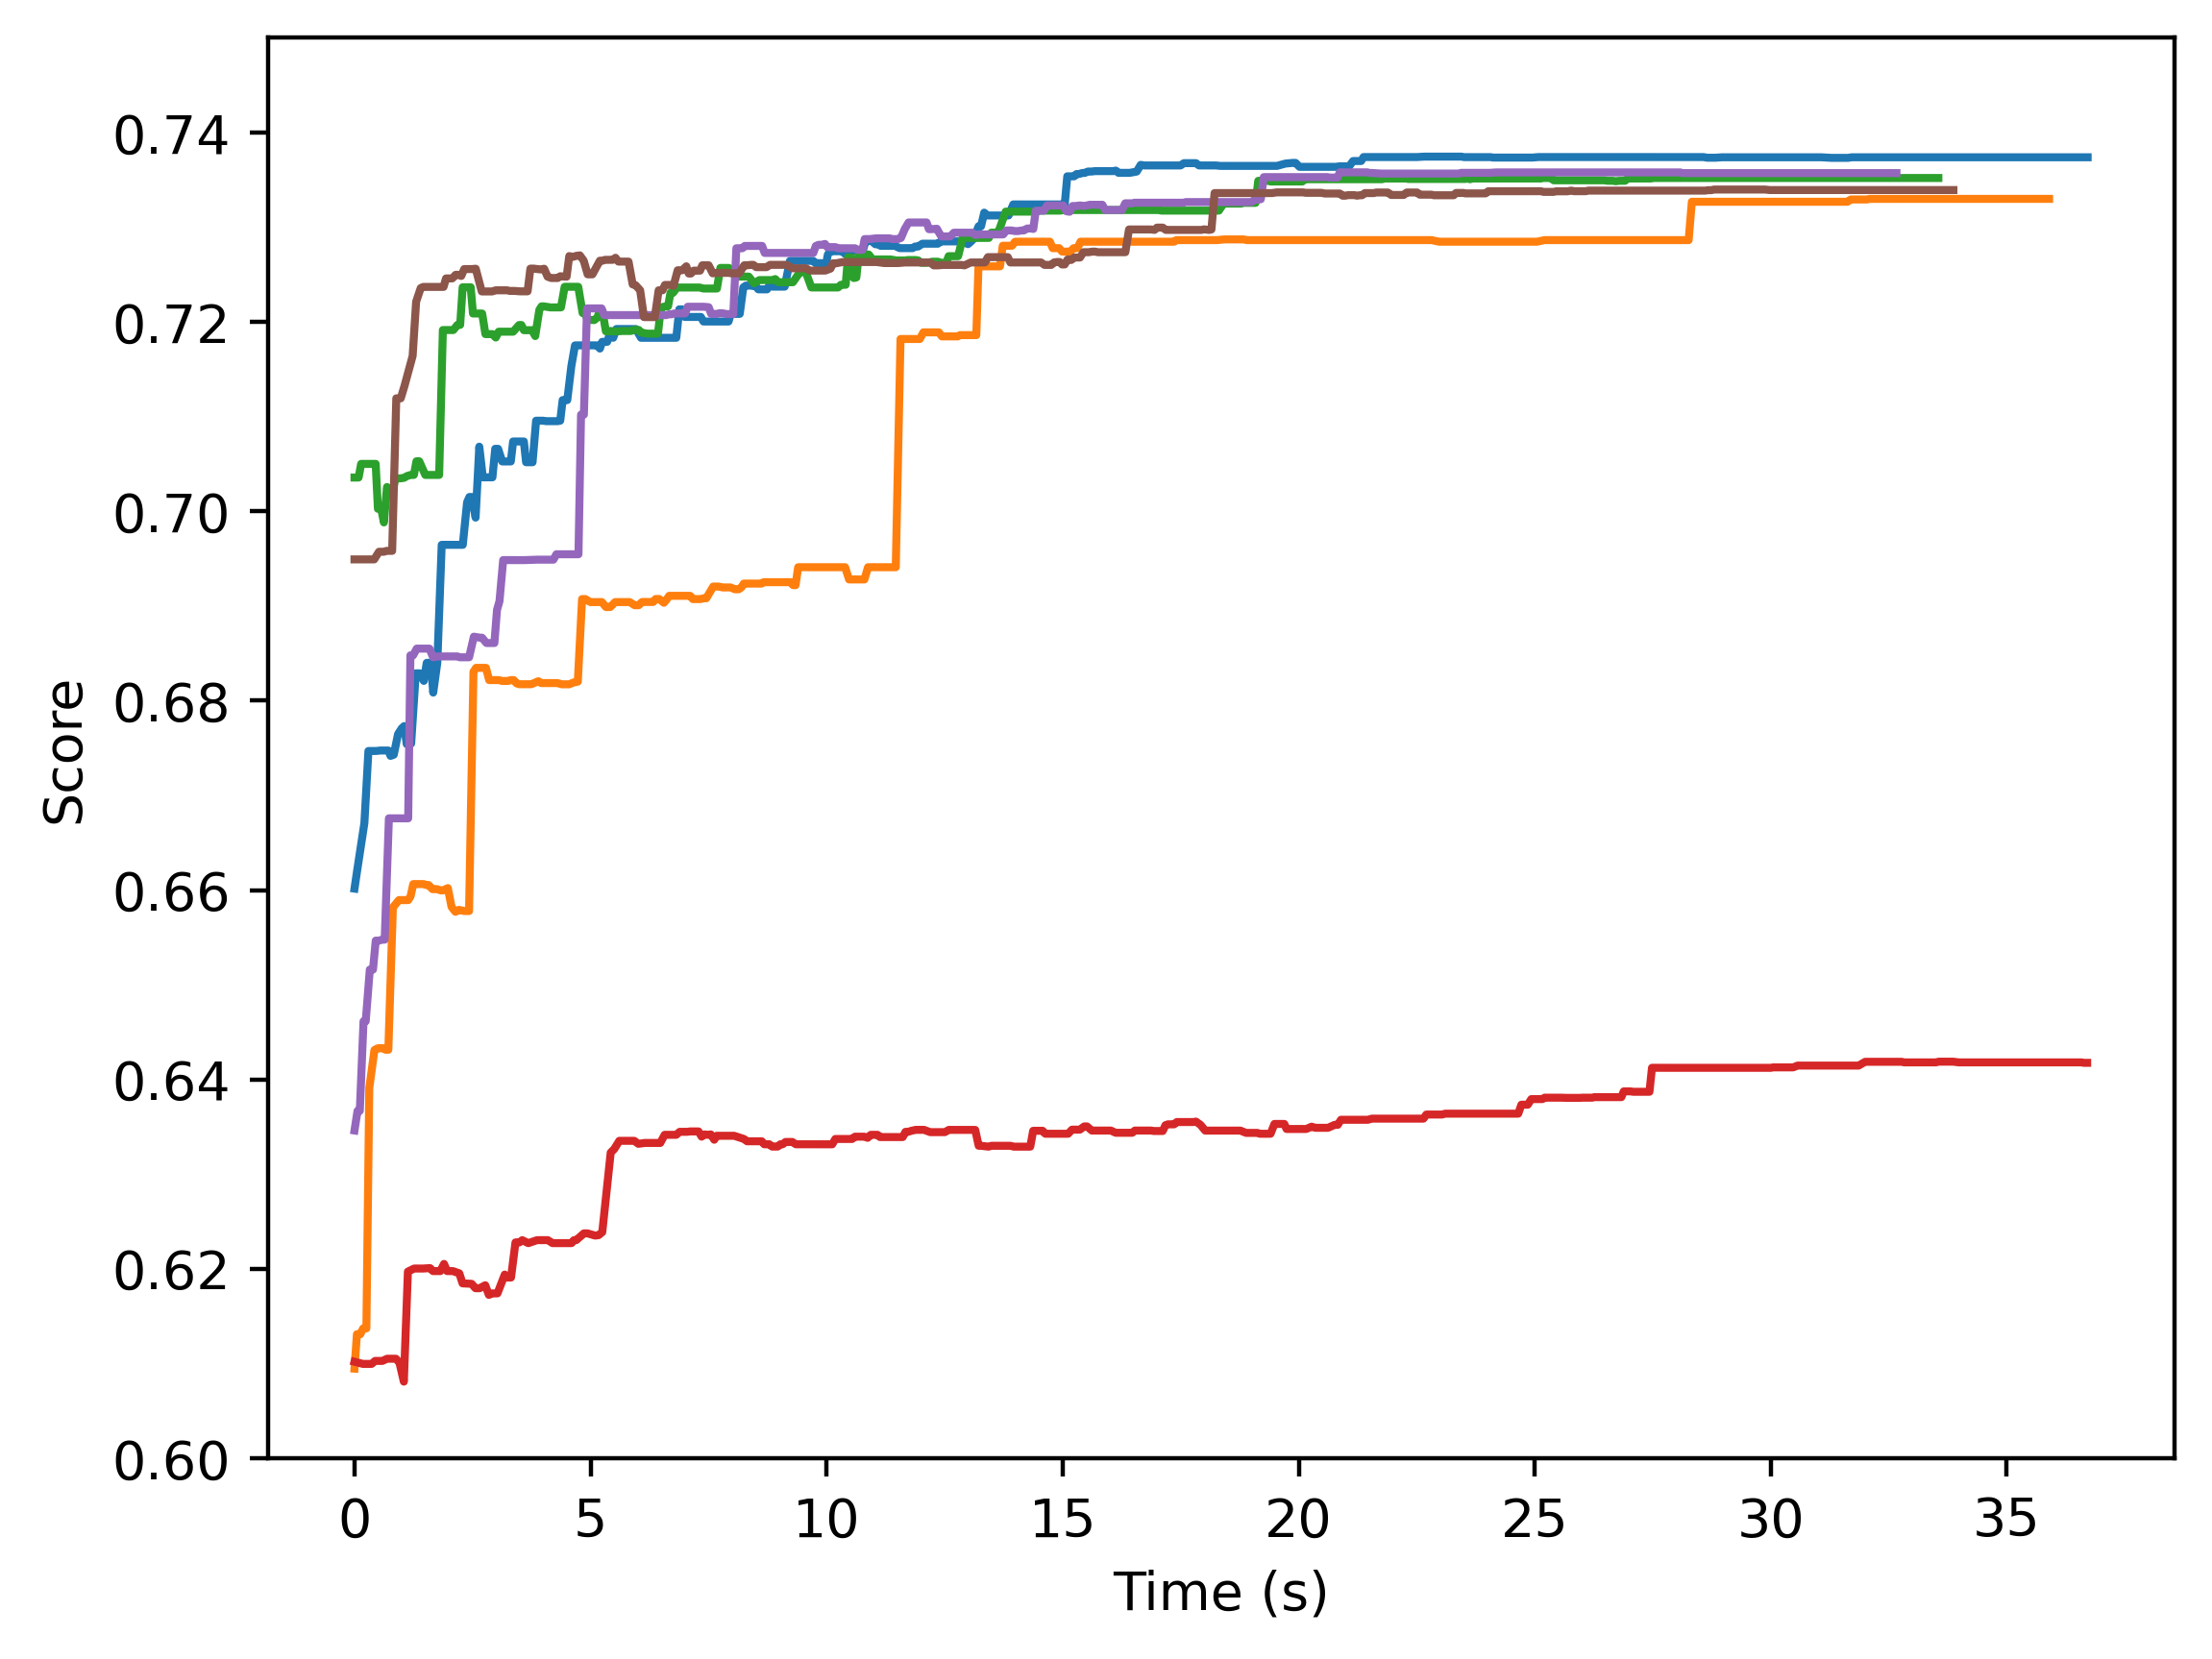
\includegraphics[width=\linewidth]{img/switchstate_exploring/suburb2/annealing_sampling/over_time.png}
      \caption{
      }
      \label{fig:annealing:over_time}
    \end{subfigure}
    \caption{
        (a) The 4 highest scoring switch states reached after annealing. Best overall
        scores and switch states from runs shown in \autoref{fig:annealing:parameters} taken.
        Layout produced with
        Kamada-Kawai layout algorithm\autocite{kamada_kawai}.\\
        (b) Scores reached through simulated annealing after a running the
        algorithm for some time. 6 samples. $\gamma = 400$, $\alpha = 0.99$ and $p_{multi} = 0.33$
    }
\end{figure}


    
